\documentclass[xcolor=dvipsnames,10pt]{beamer}

\usetheme[presnum=01]{u18fest}
\usepackage{url}
\usepackage{listings}
\usepackage{pgfplots}
\usetikzlibrary{positioning,calc}

\lstset{basicstyle=\ttfamily,breaklines=true}

\subtitle{Marco Bayesiano para el análisis de datos,\\
calibración de parámetros y modelamiento inverso}
\title{Introducción}
\institute{Universidad Industrial de Santander}
\date{U18 Fest}

\begin{document}

\begin{frame}[noframenumbering]
  \titlepage
\end{frame}

\begin{frame}
  \frametitle{Introducción}

  \textbf{David A. Barajas-Solano}
  \begin{itemize}
  \item Egresado de la UIS -- Ingeniería Civil
  \item Ph.D. en ciencias de la ingeniería, UC San Diego
  \item Científico en Pacific Northwest National Laboratory
  \item Perfil científico en \url{https://www.dbarajassolano.com}
  \end{itemize}
  
\end{frame}
%
\begin{frame}
  \frametitle{Modelamiento en ciencia e ingeniería}

  \begin{itemize}
  \item \emph{Modelos} son objetos matemáticos usados para describir fenómenos en ciencia e ingeniería
  \item Los modelos son \emph{calibrados} utilizando datos experimentales
  \end{itemize}
\end{frame}
%
\begin{frame}
  \frametitle{Modelamiento en ciencia e ingeniería}
  \begin{figure}[h]
    \centering
    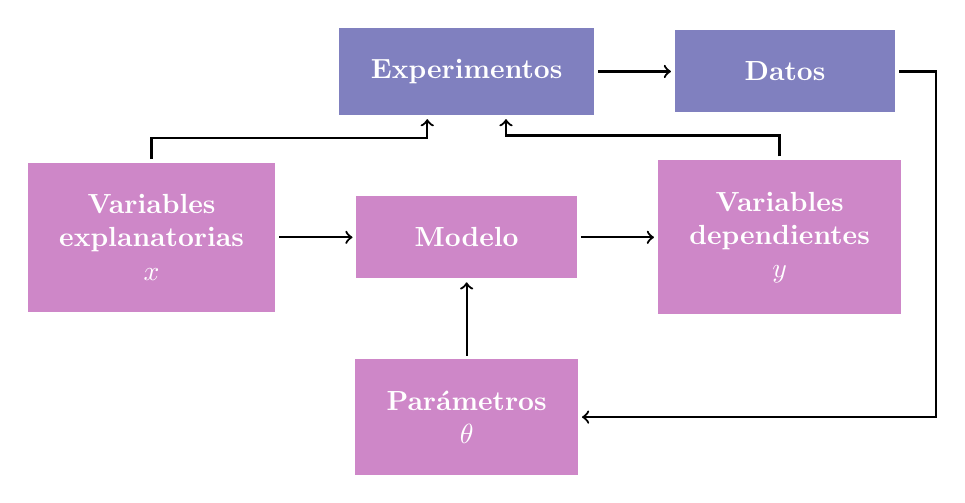
\begin{tikzpicture}[every node/.style={shape=rectangle, color=white, font=\bfseries, minimum width=2.8cm, align=center, inner sep=4mm}, every path/.style={thick, shorten >= 1pt, shorten <= 1pt}]
      \node [fill=Mulberry!50!white] (x) {Variables\\explanatorias\\$x$};%
      \node [fill=Mulberry!50!white, right=of x] (modelo) {Modelo};%
      \node [fill=Mulberry!50!white, below=of modelo] (pars) {Parámetros\\$\theta$};%
      \node [fill=Mulberry!50!white, right=of modelo] (y) {Variables\\dependientes\\$y$};%
      \node [fill=NavyBlue!50!white, above=of modelo] (exp) {Experimentos};%
      \node [fill=NavyBlue!50!white, right=of exp] (datos) {Datos};%
      \draw [->] (y.north) |- ($(y.north) + (0, 0.3cm)$) -| ($(exp.south) + (0.5cm, 0)$);%
      \draw [->] (x.north) |- ($(x.north) + (0, 0.3cm)$) -| ($(exp.south) - (0.5cm, 0)$);%
      \draw [->] (datos.east) -| ($(datos.east) + (0.5cm, 0cm)$) |- (pars.east);%
      \draw [->] (x) -- (modelo);%
      \draw [->] (modelo) -- (y);%
      \draw [->] (pars) -- (modelo);%
      \draw [->] (exp) -- (datos);%
    \end{tikzpicture}
  \end{figure}
\end{frame}
%
\begin{frame}
  \frametitle{Ejemplos de modelos}
  \begin{itemize}
  \item \emph{Ley de Hooke}
    \begin{equation*}
      \sigma = E \varepsilon
    \end{equation*}
    \vspace{-\baselineskip}
    \begin{itemize}
    \item Parámetros: Módulo de Young $E$
    \end{itemize}
    \pause
  \item \emph{Leyes de reacción}
    \begin{equation*}
      R = k [A] [B]
    \end{equation*}
    \vspace{-\baselineskip}
    \begin{itemize}
    \item Observaciones indirectas e.g. respuesta química vs tiempo
    \item Parámetros: Tasa de reacción $k$
    \end{itemize}
    \pause
  \item \emph{Modelo logístico para variables categóricas}
    \begin{equation*}
      \log \frac{P(y = 1)}{P(y = 0)} = \alpha + \beta x
    \end{equation*}
    \vspace{-\baselineskip}
    \begin{itemize}
    \item Variable categórica dependiente $y = {0, 1}$
    \item Variable explanatoria contínua $x$
    \item Parámetros $\theta = {\alpha, \beta}$
    \end{itemize}
  \end{itemize}
\end{frame}
%
\begin{frame}
  \frametitle{Objetivos}
  \begin{itemize}
  \item \textbf{Modelamiento \emph{probabilístico} para la selección, calibración, y evaluación de modelos científicos}
    \begin{itemize}
    \item \emph{Selección}: Cuál modelo utilizar?
    \item \emph{Calibración}: Qué valores utilizar para los parámetros?
    \item \emph{Evaluación}: Es el modelo calibrado útil?
    \end{itemize}
  \item \emph{Marco Bayesiano} para modelamiento probabilístico
  \item \emph{Programación probabilística} para la práctica
  \item Algunos modelos sencillos con aplicaciones
  \end{itemize}
\end{frame}
%
\begin{frame}
  \frametitle{Programa}
  \begin{tcolorbox}[title=Fundamentos]
    \begin{itemize}
    \item \emph{Lunes}: Teoría de la probabilidad y teorema de Bayes
    \item \emph{Martes}: Modelamiento y programación probabilística
    \end{itemize}
  \end{tcolorbox}
  \begin{tcolorbox}[title=Regresión]
    \begin{itemize}
    \item \emph{Martes}: Modelos lineales
    \item \emph{Miércoles}: Modelos no lineales
    \item \emph{Jueves}: Modelos jierárquicos
    \end{itemize}
  \end{tcolorbox}
\end{frame}
%
\begin{frame}
  \frametitle{Metodología}
  \begin{itemize}
  \item Vamos a programar? \textbf{No}, pero...
  \item ...vamos a utilizar herrramientas de programación probabilística para explorar conceptos
  \end{itemize}
  \textbf{Herramientas de programación basadas en texto plano}
  \begin{itemize}
  \item Lenguaje de programación \textsf{Python}
  \item Librería de programación probabilística \textsf{PyMC3}
  \item Interfase de cuadernos \textsf{Jupyter Lab}
  \end{itemize}
\end{frame}
%
\begin{frame}[fragile]
  \frametitle{Programación basada en texto plano}
  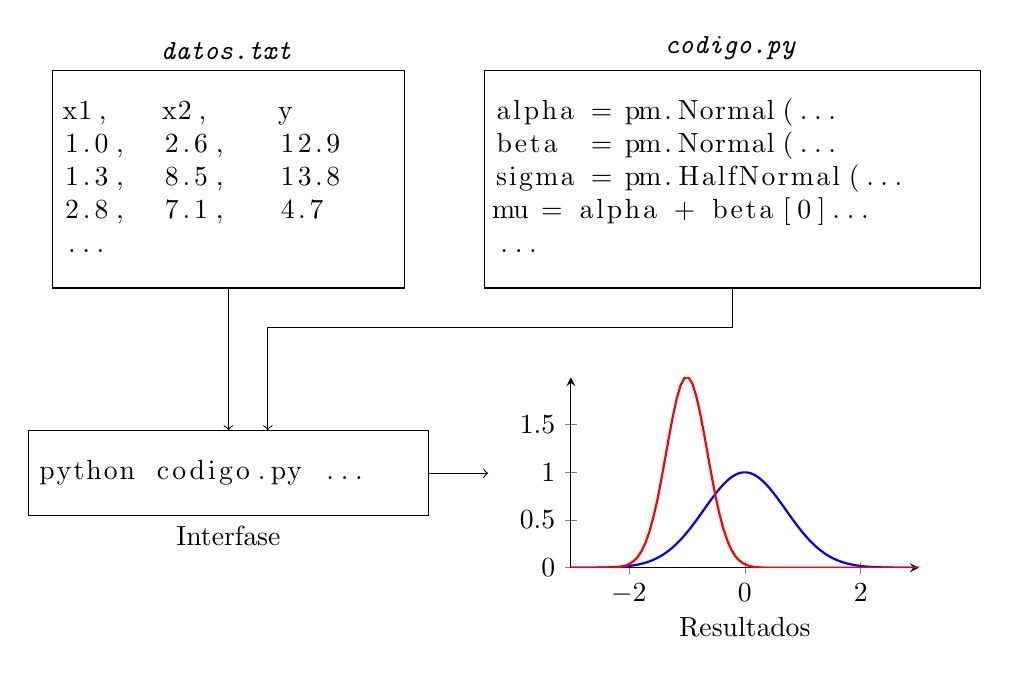
\begin{tikzpicture}[node distance=1.8cm and 1cm]
    \node [shape=rectangle, draw, label=above:{\textit{\texttt{datos.txt}}}] (datos) {%
      \begin{minipage}{0.35\textwidth}
        \begin{lstlisting}[language=python]
x1,   x2,    y
1.0,  2.6,   12.9   
1.3,  8.5,   13.8
2.8,  7.1,   4.7
...
        \end{lstlisting}
      \end{minipage}
    };
    \node [shape=rectangle, draw, label=above:{\textit{\texttt{codigo.py}}}, right=of datos] (codigo) {%
      \begin{minipage}{0.5\textwidth}
        \begin{lstlisting}[language=python]
alpha = pm.Normal(...
beta  = pm.Normal(...
sigma = pm.HalfNormal(...
mu = alpha + beta[0]...
...
        \end{lstlisting}
      \end{minipage}
    };
    \node [shape=rectangle, draw, label=below:Interfase, below=of datos] (cli) {%
      \begin{minipage}{0.4\textwidth}
        \begin{lstlisting}[language=sh]
python codigo.py ...
        \end{lstlisting}
      \end{minipage}
    };%
    \begin{axis}[xmin=-3, xmax=3, height=4cm, width=6cm, axis x line=middle, axis y line=left, at={($(cli.east)+(1.8cm, -1.2cm)$)}, title=Resultados, title style={at={(0.5,-0.5)}}]
      \addplot [samples=150, no markers, blue, thick] {exp{-x^2}};%
      \addplot [samples=150, no markers, red,  thick] {2*exp{-(x+1)^2 * 4}};%
    \end{axis}
    \draw [->] (datos)--(cli);
    \draw [->] (codigo.south) |- ($(codigo.south) - (0, 0.5cm)$) -| ($(cli.north) + (0.5cm, 0)$);
    \draw [->] (cli) -- node {} ($(cli.east) + (0.75cm, 0)$);
  \end{tikzpicture}
\end{frame}
%
\begin{frame}
  \frametitle{Programación basada en texto plano}
  \textbf{Ventajas}
  \begin{itemize}
  \item \emph{Reproducibilidad}: Se puede recrear mi análisis y resultados?
  \item \emph{Transparencia}: Se puede ver cómo el análisis se ha hecho?
  \item \emph{Mantenibilidad}: Se puede acceder, cambiar, o actualizar el análisis?
  \end{itemize}
  \textbf{Alternativas}
  \begin{itemize}
  \item Software de oficina
  \end{itemize}
\end{frame}
%
\begin{frame}
  \frametitle{Ejemplo: Éste taller!}
  \begin{itemize}
  \item \emph{Reproducibilidad}: Software libre para generar todo el contenido (presentaciones, máquina virtual, cuadernos, etc.)
  \item \emph{Transparencia}: Texto plano es transparente
  \item \emph{Mantenibilidad}: Via \textsf{Git}
  \end{itemize}
\end{frame}
%
\begin{frame}
  \frametitle{Logística}
  \begin{itemize}
  \item Cronograma
    \begin{itemize}
    \item Dos mitades de 1h 20m
    \item Pausa de 20m entre mitades (café y aromáticas afuera)
    \end{itemize}
  \item Código, cuadernos y presentaciones disponibles en \textsf{GitHub}\\
    \url{https://github.com/dbarajassolano/u18fest}
  \item \textbf{Preguntas bienvenidas a cualquier momento!}
  \end{itemize}
\end{frame}

\end{document}

%%% Local Variables:
%%% TeX-master: t
%%% TeX-engine: luatex
%%% ispell-local-dictionary: "spanish"
%%% End:
